\documentclass{article}

% content/resources/templates/preamble.tex
\usepackage[margin=0.6in]{geometry}
\author{Milav Dabgar}
\usepackage{amsmath,amssymb,amsthm}
\usepackage{booktabs}
\usepackage{multirow}
\usepackage{xcolor}
\usepackage{tcolorbox}
\tcbuselibrary{breakable,skins}
\usepackage[colorlinks=true,linkcolor=blue]{hyperref}
\usepackage{titlesec}
\usepackage{enumitem}
\usepackage{tikz}
\usepackage{pgfplots}
\usepackage{circuitikz}
\usepackage[version=4]{mhchem}
\usepackage{longtable}
\usepackage{array}
\usepackage{float}
\usepackage{caption}
\usepackage{listings}

\lstset{
  basicstyle=\small\ttfamily,
  breaklines=true,
  breakatwhitespace=false,
  postbreak=\mbox{\textcolor{red}{$\hookrightarrow$}\space},
  float=false,
  numbers=left,
  numberstyle=\tiny\color{gray},
  numbersep=10pt,
  xleftmargin=2em,
  keywordstyle=\color{blue},
  commentstyle=\color{green!60!black},
  stringstyle=\color{purple},
  backgroundcolor=\color{gray!5},
  showstringspaces=false,
  tabsize=2,
  captionpos=b,
  keepspaces=true,
  columns=flexible
}

\pgfplotsset{compat=1.18}
\usetikzlibrary{shapes,arrows,positioning,calc,patterns,decorations.pathmorphing,decorations.markings,arrows.meta}

% Color scheme
\definecolor{headcolor}{RGB}{0,102,204}
\definecolor{keycolor}{RGB}{220,20,60}
\definecolor{solutioncolor}{RGB}{34,139,34}
\definecolor{mnemoniccolor}{RGB}{148,0,211}
\definecolor{codecolor}{RGB}{0,0,100}

% Spacing
\setlength{\parskip}{3pt}
\setlist[itemize]{nosep}
\setlist[enumerate]{nosep}

% Title formatting
\titleformat{\section}{\Large\bfseries\color{headcolor}}{\thesection}{1em}{}
\titleformat{\subsection}{\large\bfseries\color{headcolor}}{\thesubsection}{1em}{}

% Pandoc tightlist compatibility
\providecommand{\tightlist}{%
  \setlength{\itemsep}{0pt}\setlength{\parskip}{0pt}}

% Pandoc longtable compatibility
\newcounter{none}
\def\thenone{}


% content/resources/templates/english-boxes.tex

% Custom environments
\newtcolorbox{solutionbox}{
 breakable,
 enhanced,
 colback=solutioncolor!5!white,
 colframe=solutioncolor!75!black,
 fonttitle=\bfseries,
 title=Solution
}

\newtcolorbox{solutionboxnobreak}{
 colback=solutioncolor!5!white,
 colframe=solutioncolor!75!black,
 fonttitle=\bfseries,
 title=Solution
}

\newtcolorbox{keyformula}{
 breakable,
 enhanced,
 colback=keycolor!5!white,
 colframe=keycolor!75!black,
 fonttitle=\bfseries,
 title=Key Formula
}

\newtcolorbox{mnemonicboxenv}{
 breakable,
 enhanced,
 colback=mnemoniccolor!5!white,
 colframe=mnemoniccolor!75!black,
 fonttitle=\bfseries,
 title=Mnemonic
}

\newcommand{\mnemonicbox}[1]{%
  \begin{mnemonicboxenv}
    #1
  \end{mnemonicboxenv}
}


% Custom commands for GTU solutions
% This file defines semantic commands for consistent formatting

% Question command with automatic formatting
\newcommand{\question}[2]{%
  \section*{Question #1}%
  \textbf{#2}%
}

% OR question variant
\newcommand{\questionor}[2]{%
  \section*{Question #1 OR}%
  \textbf{#2}%
}

% Proper table environment with caption
\newenvironment{answertable}[1]{%
  \begin{table}[htbp]
  \centering
  \caption{#1}
}{%
  \end{table}
}

% Proper figure environment for diagrams
\newenvironment{answerdiagram}[1]{%
  \begin{figure}[htbp]
  \centering
  \caption{#1}
}{%
  \end{figure}
}

% Semantic markup for key terms
\newcommand{\keyword}[1]{\textbf{#1}}
\newcommand{\code}[1]{\texttt{#1}}
\newcommand{\classname}[1]{\texttt{#1}}
\newcommand{\methodname}[1]{\texttt{#1}}

% Proper quotation marks
\newcommand{\mnemonic}[1]{``#1''}


\title{Electronics Devices \& Circuits (1323202) - Summer 2024 Solution}
\date{June 21, 2024}

\begin{document}
\maketitle

\questionmarks{1(a)}{3}{What is heat sink. lists its types}

\begin{solutionbox}
A heat sink is a passive device that absorbs and dissipates heat from electronic components to prevent overheating.

\begin{center}
\captionof{table}{Types of Heat Sinks}
\begin{tabulary}{\linewidth}{|L|L|}
\hline
\textbf{Type} & \textbf{Description} \\
\hline
\textbf{Passive} & Uses natural convection without external power \\
\hline
\textbf{Active} & Incorporates fans or liquid cooling \\
\hline
\textbf{Radial} & Fins arranged in radial pattern from center \\
\hline
\textbf{Pin-fin} & Uses pins or rods for increased surface area \\
\hline
\textbf{Extruded} & Made by forcing aluminum through shaped die \\
\hline
\end{tabulary}
\end{center}

\begin{mnemonicbox}
"PAPER" (Passive, Active, Pin-fin, Extruded, Radial)
\end{mnemonicbox}
\end{solutionbox}

\questionmarks{1(b)}{4}{Define the Following: 1. Thermal Runaway 2. Thermal Stability}

\begin{solutionbox}
\textbf{Thermal Runaway}:
The self-accelerating destructive process where increased temperature causes increased current flow, which further increases temperature, potentially destroying the transistor.

\textbf{Thermal Stability}:
The ability of a transistor circuit to maintain stable operation despite temperature changes, preventing thermal runaway.

\begin{center}
\begin{tikzpicture}[gtu block]
    \node (temp) [draw, rectangle] {Temperature Rises};
    \node (ic) [draw, rectangle, right=1cm of temp] {Collector Current Increases};
    \node (pd) [draw, rectangle, right=1cm of ic] {Power Dissipation Increases};
    \node (dest) [draw, rectangle, below=1cm of temp] {Device Destruction};
    
    \draw [gtu arrow] (temp) -- (ic);
    \draw [gtu arrow] (ic) -- (pd);
    \draw [gtu arrow] (pd.south) -- ++(0,-0.5) -| (temp.south);
    \draw [gtu arrow] (temp) -- (dest);
\end{tikzpicture}
\end{center}

\begin{mnemonicbox}
"RISE" (Runaway Is Self-Escalating)
\end{mnemonicbox}
\end{solutionbox}

\questionmarks{1(c)}{7}{Explain voltage divider bias in details.}

\begin{solutionbox}
Voltage divider bias is a common transistor biasing technique that provides stable operation.

\begin{center}
\begin{circuitikz}[american]
    \draw (0,0) node[ground] {} to[R, l=$R_E$] (0,2) -- (0,2.5) node[npn, anchor=E] (Q) {};
    \draw (Q.C) -- (0,4.5) to[R, l=$R_C$] (0,6.5) -- (0,7) node[vcc] {$+V_{CC}$};
    \draw (Q.B) -- (-1.5, 3.25);
    \draw (-1.5, 3.25) to[R, l=$R_2$, *-] (-1.5, 0) node[ground] {};
    \draw (-1.5, 3.25) to[R, l=$R_1$] (-1.5, 7) node[vcc] {$+V_{CC}$};
    
    % \draw (-1.5, 7) -- (0, 7); % Connect VCC
\end{circuitikz}
\end{center}

\begin{itemize}
    \item \textbf{Voltage divider network}: $R_1$ and $R_2$ establish a fixed base voltage
    \item \textbf{Stable Q-point}: Maintains operating point despite temperature variations
    \item \textbf{Better stability}: Higher stability factor compared to fixed bias
    \item \textbf{Self-adjusting}: Base current automatically adjusts to counter temperature changes
\end{itemize}

\begin{mnemonicbox}
"VSST" (Voltage divider, Stable, Self-adjusting, Temperature resistant)
\end{mnemonicbox}
\end{solutionbox}

\vspace{0.5em}\centerline{\textbf{OR}}\questionmarks{1(c)}{7}{Explain D.C. Load Line in details.}

\begin{solutionbox}
DC Load Line is a graphical method for analyzing transistor bias conditions.

\begin{center}
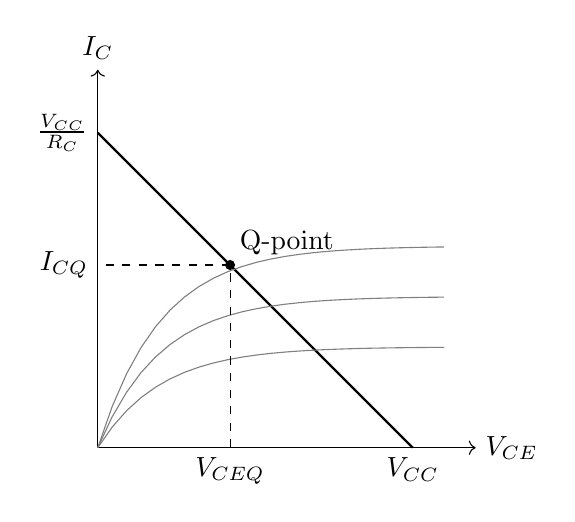
\begin{tikzpicture}[scale=0.8]
    % Axes
    \draw[->] (0,0) -- (6,0) node[right] {$V_{CE}$};
    \draw[->] (0,0) -- (0,6) node[above] {$I_C$};
    
    % Load Line
    \draw [thick] (0,5) node[left] {$\frac{V_{CC}}{R_C}$} -- (5,0) node[below] {$V_{CC}$};
    
    % Output Characterisitics (Simplified)
    \draw [gray, domain=0:5.5] plot (\x, {4*(1-exp(-\x))*0.8});
    \draw [gray, domain=0:5.5] plot (\x, {4*(1-exp(-\x))*0.6});
    \draw [gray, domain=0:5.5] plot (\x, {4*(1-exp(-\x))*0.4});
    
    % Q-point
    \filldraw (2.1, 2.9) circle (2pt) node[above right] {Q-point};
    \draw [dashed] (2.1, 0) node[below] {$V_{CEQ}$} -- (2.1, 2.9) -- (0, 2.9) node[left] {$I_{CQ}$};
\end{tikzpicture}
\end{center}

\begin{itemize}
    \item \textbf{Definition}: Graphical line showing all possible operating points for a given circuit
    \item \textbf{Endpoints}: $(0, V_{CC}/R_C)$ and $(V_{CC}, 0)$ on $I_C$-$V_{CE}$ plane
    \item \textbf{Q-point}: Intersection of load line with transistor characteristic curve
    \item \textbf{Equation}: $I_C = (V_{CC} - V_{CE})/R_C$
\end{itemize}

\begin{mnemonicbox}
"QECC" (Q-point Exists where Collector Current meets characteristics)
\end{mnemonicbox}
\end{solutionbox}

\questionmarks{2(a)}{3}{Explain how transistor works as a switch.}

\begin{solutionbox}
A transistor switch operates in either saturation (ON) or cutoff (OFF) regions.

\begin{center}
\captionof{table}{Transistor Switch Operation}
\begin{tabulary}{\linewidth}{|L|L|L|L|L|}
\hline
\textbf{State} & \textbf{Region} & \textbf{Base Current} & \textbf{Collector Current} & \textbf{VCE} \\
\hline
\textbf{OFF} & Cutoff & $I_B \approx 0$ & $I_C \approx 0$ & $V_{CE} \approx V_{CC}$ \\
\hline
\textbf{ON} & Saturation & $I_B > I_{B(sat)}$ & $I_C \approx I_{C(sat)}$ & $V_{CE} \approx 0.2V$ \\
\hline
\end{tabulary}
\end{center}

\begin{mnemonicbox}
"COS" (Cutoff Off, Saturation on)
\end{mnemonicbox}
\end{solutionbox}

\questionmarks{2(b)}{4}{Draw and explain colpitt oscillator.}

\begin{solutionbox}
Colpitt oscillator is an LC oscillator using a capacitive voltage divider for feedback.

\begin{center}
\begin{circuitikz}[american]
    \draw (0,0) node[ground] {} to[R, l=$R_E$] (0,2) -- (0,2.5) node[npn, anchor=E] (Q) {};
    \draw (Q.C) -- (0,4.5) to[R, l=$R_C$] (0,6.5) -- (0,7) node[vcc] {$+V_{CC}$};
    
    % Biasing
    \draw (Q.B) -- (-1.5, 3.25);
    \draw (-1.5, 3.25) to[R, l=$R_2$, *-] (-1.5, 0) node[ground] {};
    \draw (-1.5, 3.25) to[R, l=$R_1$] (-1.5, 7) node[vcc] {$+V_{CC}$};
    
    % Tank Circuit
    \draw (Q.C) to[C, l=$C_3$] (3, 4.5) -- (3, 3.25);
    \draw (3, 3.25) to[L, l=$L$, *-*] (3, 0) node[ground] {};
    \draw (3, 3.25) -- (5, 3.25) to[C, l=$C_1$] (5, 1.625) to[C, l=$C_2$, *-] (5, 0) node[ground] {}; 
    \draw (5, 3.25) -- (5, 4.5) -- (Q.C); % Feedback from C (Corrected below)
    
    % Correct Colpitts feedback:
    % Inductor in parallel with two series capacitors.
    % Feedback taken from junction of C1 and C2 to Emitter usually, or Base.
    % Basic Circuit: L // (C1 + C2)
    % Let's draw standard tank
    \draw (2.5, 4.5) to[short, *-] (4.5, 4.5) to[C, l=$C_1$] (4.5, 2.5) to[short, *-] (2.5, 2.5) to[L, l=$L$] (2.5, 4.5);
    \draw (4.5, 2.5) to[C, l=$C_2$] (4.5, 0.5) node[ground] {};
    \draw (Q.C) to[short] (2.5, 4.5); % Output to Tank
    \draw (4.5, 4.5) -- (5.5, 4.5) -- (5.5, 3.25) -- (-1.5, 3.25); % Feedback to Base
    % Actually feedback in Colpitts is often C1-C2 split. 
\end{circuitikz}
% Simplified Diagram for exam clarity
\begin{circuitikz}[american, scale=0.9, transform shape]
    \node [npn] (Q) at (0,0) {};
    \draw (Q.E) to[R, l=$R_E$] ++(0,-2) node[ground]{};
    \draw (Q.C) to[R, l=$R_C$] ++(0,2) node[vcc]{$+V_{CC}$};
    \draw (Q.B) to[R, l=$R_2$] ++(0,-2) node[ground]{};
    \draw (Q.B) to[R, l=$R_1$] ++(0,2) node[vcc]{$+V_{CC}$};
    
    % Tank
    \draw (Q.C) to[C, l=$C_{out}$] (3,0.77);
    \draw (3,0.77) to[L, l=$L$] (3,-2) node[ground]{};
    \draw (3,0.77) -- (5,0.77) to[C, l=$C_1$] (5,-0.6) to[C, l=$C_2$] (5,-2) node[ground]{};
    \draw (5,-0.6) -- (5,-0.6) to[short] (5,-1) -- (-2,-1) -- (-2,0) -- (Q.B); % Feedback
\end{circuitikz}
\end{center}

\begin{itemize}
    \item \textbf{Feedback}: Provided by capacitive voltage divider ($C_1$, $C_2$)
    \item \textbf{Resonant frequency}: $f = 1/(2\pi\sqrt{L \times C})$, where $C = (C_1 \times C_2)/(C_1+C_2)$
    \item \textbf{Oscillation}: Maintains through regenerative feedback
    \item \textbf{Phase shift}: 360\degree around the loop
\end{itemize}

\begin{mnemonicbox}
"CFPO" (Capacitive Feedback Produces Oscillations)
\end{mnemonicbox}
\end{solutionbox}

\questionmarks{2(c)}{7}{Explain Frequency Response Two Stage RC Coupled Amplifier with circuit diagram.}

\begin{solutionbox}
Two-stage RC coupled amplifier combines two amplifier stages with RC coupling.

\begin{center}
\begin{circuitikz}[american, scale=0.8, transform shape]
    % Stage 1
    \node [npn] (Q1) at (0,0) {$Q_1$};
    \draw (Q1.E) to[R, l=$R_{E1}$] (0,-2) node[ground]{};
    \draw (Q1.C) to[R, l=$R_{C1}$] (0,2) node[vcc](VCC){$+V_{CC}$};
    \draw (Q1.B) to[short] (-1,0); 
    \draw (-1,0) to[R, l=$R_{2}$] (-1,-2) node[ground]{};
    \draw (-1,0) to[R, l=$R_{1}$] (-1,2) node[vcc]{};
    \draw (-1,0) to[C, l=$C_{in}$] (-3,0) node[left]{$V_{in}$};
    
    % Coupling
    \draw (Q1.C) to[C, l=$C_C$] (2,0);
    
    % Stage 2
    \node [npn] (Q2) at (3,0) {$Q_2$};
    \draw (Q2.E) to[R, l=$R_{E2}$] (3,-2) node[ground]{};
    \draw (Q2.C) to[R, l=$R_{C2}$] (3,2) node[vcc]{};
    \draw (Q2.B) to[short] (2,0);
    \draw (2,0) to[R, l=$R_{4}$] (2,-2) node[ground]{};
    \draw (2,0) to[R, l=$R_{3}$] (2,2) node[vcc]{};
    \draw (Q2.C) to[C, l=$C_{out}$] (5,0) node[right]{$V_{out}$};
\end{circuitikz}
\end{center}

\textbf{Frequency Response:}
\begin{center}
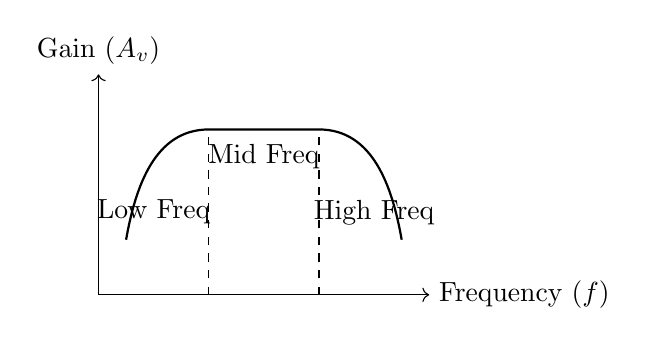
\begin{tikzpicture}[scale=0.7]
    \draw[->] (0,0) -- (6,0) node[right] {Frequency ($f$)};
    \draw[->] (0,0) -- (0,4) node[above] {Gain ($A_v$)};
    
    \draw[thick] (0.5,1) to[out=80,in=180] (2,3) to[short] (4,3) to[out=0,in=100] (5.5,1);
    
    \draw[dashed] (2,0) -- (2,3);
    \draw[dashed] (4,0) -- (4,3);
    
    \node at (1,1.5) {Low Freq};
    \node at (3,2.5) {Mid Freq};
    \node at (5,1.5) {High Freq};
\end{tikzpicture}
\end{center}

\begin{itemize}
    \item \textbf{Low frequency}: Gain drops due to coupling capacitor impedance
    \item \textbf{Mid frequency}: Maximum flat gain region (bandwidth)
    \item \textbf{High frequency}: Gain drops due to transistor capacitance effects
    \item \textbf{Overall gain}: Product of individual stage gains
\end{itemize}

\begin{mnemonicbox}
"LMH" (Low drops, Mid flat, High drops)
\end{mnemonicbox}
\end{solutionbox}

\vspace{0.5em}\centerline{\textbf{OR}}\questionmarks{2(a)}{3}{Draw circuit diagram of Hartley oscillator.}

\begin{solutionbox}
\begin{center}
\captionof{figure}{Hartley Oscillator}
\begin{circuitikz}[american, scale=0.9, transform shape]
    \node [npn] (Q) at (0,0) {};
    \draw (Q.E) to[R, l=$R_E$] ++(0,-2) node[ground]{};
    \draw (Q.C) to[R, l=$R_C$] ++(0,2) node[vcc]{$+V_{CC}$};
    \draw (Q.B) to[R, l=$R_2$] ++(0,-2) node[ground]{};
    \draw (Q.B) to[R, l=$R_1$] ++(0,2) node[vcc]{};
    
    % Tank
    \draw (Q.C) to[C, l=$C_{out}$] (3,0.77);
    \draw (3,0.77) to[C, l=$C$] (3,-2) node[ground]{};
    \draw (3,0.77) -- (5,0.77) to[L, l=$L_1$] (5,-0.6) to[L, l=$L_2$] (5,-2) node[ground]{};
    \draw (5,-0.6) -- (5,-0.6) to[short] (5,-1) -- (-2,-1) -- (-2,0) -- (Q.B); % Feedback
\end{circuitikz}
\end{center}

\begin{mnemonicbox}
"ITLC" (Inductor Tapped for LC Circuit)
\end{mnemonicbox}
\end{solutionbox}

\questionmarks{2(b)}{4}{List different types of negative feedback.}

\begin{solutionbox}
\begin{center}
\captionof{table}{Types of Negative Feedback}
\begin{tabulary}{\linewidth}{|L|L|L|}
\hline
\textbf{Type} & \textbf{Configuration} & \textbf{Effect on Parameters} \\
\hline
\textbf{Voltage Series} & Output voltage fed to input in series & Increases input impedance, reduces distortion \\
\hline
\textbf{Voltage Shunt} & Output voltage fed to input in parallel & Decreases input impedance, increases bandwidth \\
\hline
\textbf{Current Series} & Output current fed to input in series & Increases output impedance, stabilizes current gain \\
\hline
\textbf{Current Shunt} & Output current fed to input in parallel & Decreases output impedance, stabilizes voltage gain \\
\hline
\end{tabulary}
\end{center}

\begin{mnemonicbox}
"VSCS" (Voltage Series, Current Shunt)
\end{mnemonicbox}
\end{solutionbox}

\questionmarks{2(c)}{7}{List advantages of Negative feedback amplifier and Explain voltage series negative feedback in details.}

\begin{solutionbox}
\textbf{Advantages of Negative Feedback:}
\begin{itemize}
    \item Stabilizes gain against component variations
    \item Reduces distortion and noise
    \item Increases bandwidth
    \item Modifies input/output impedance
    \item Improves linearity
\end{itemize}

\textbf{Voltage Series Negative Feedback:}

\begin{center}
\begin{tikzpicture}[gtu block]
    \node (sum) [draw, circle] {$\Sigma$};
    \node (amp) [draw, rectangle, right=1cm of sum] {Amplifier A};
    \node (fb) [draw, rectangle, below=1cm of amp] {Feedback Network $\beta$};
    
    \draw [gtu arrow] (sum) -- (amp);
    \draw [gtu arrow] (amp) -- (4,0) node[right] {$V_{out}$};
    \draw [gtu arrow] (3.5,0) |- (fb);
    \draw [gtu arrow] (fb) -| (sum);
    \draw [gtu arrow] (-1,0) node[left] {$V_{in}$} -- (sum);
\end{tikzpicture}
\end{center}

\begin{itemize}
    \item \textbf{Configuration}: Output voltage sampled, fed back in series with input
    \item \textbf{Closed-loop gain}: $A_{CL} = A/(1+A\beta)$, where A is open-loop gain and $\beta$ is feedback fraction
    \item \textbf{Input impedance}: Increases by factor $(1+A\beta)$
    \item \textbf{Output impedance}: Decreases by factor $(1+A\beta)$
\end{itemize}

\begin{mnemonicbox}
"SIGO" (Stable gain, Increased input impedance, Gain reduction, Output impedance reduction)
\end{mnemonicbox}
\end{solutionbox}
\questionmarks{3(a)}{3}{Draw circuit of SCR using two transistor analogy.}

\begin{solutionbox}
\textbf{Two Transistor Analogy of SCR:}

\begin{center}
\begin{circuitikz}[american, scale=0.8, transform shape]
    % PNP Transistor (Q1)
    \node [pnp, rotate=0] (Q1) at (0,2) {$Q_1$};
    % NPN Transistor (Q2)
    \node [npn, rotate=0] (Q2) at (2,0) {$Q_2$};
    
    % Connections
    \draw (Q1.E) to[short] (0,4) node[above] {Anode (A)};
    \draw (Q2.E) to[short] (2,-2) node[below] {Cathode (K)};
    
    % Collector Q1 to Base Q2
    \draw (Q1.C) -- (0,0) -- (Q2.B);
    
    % Base Q1 to Collector Q2
    \draw (Q1.B) -- (2,2) -- (Q2.C);
    
    % Gate connection to Base of Q2 (Standard) or Base Q2
    % Actually Gate is connected to P-layer of NPN base usually (P2)
    % Diagram shows G to B2 (Base NPN) based on MDX diagram description:
    % E1[Emitter PNP] --- B2[Base NPN] ? Wait.
    % MDX Graph:
    % A --- C1
    % C1 --- E2
    % E2 --- K
    % E1 --- B2 (Wait, Emitter of PNP connected to Base of NPN? No that's latch up)
    % Standard Analogy:
    % PNP (Q1): Emitter=Anode, Base=Connected to Collector Q2, Collector=Connected to Base Q2
    % NPN (Q2): Collector=Connected to Base Q1, Base=Connected to Collector Q1, Emitter=Cathode
    % Gate connected to Base of Q2 (NPN)
    
    \draw (Q2.B) to[short, -o] (-1,0) node[left] {Gate (G)};
    
    % Correcting connections based on standard theory
    % PNP Collector -> NPN Base
    % NPN Collector -> PNP Base
\end{circuitikz}
\end{center}

\begin{mnemonicbox}
"PNPNPN" (PNP and NPN structure)
\end{mnemonicbox}
\end{solutionbox}

\questionmarks{3(b)}{4}{Draw and explain Natural Commutation of SCR.}

\begin{solutionbox}
Natural commutation occurs when the SCR current naturally falls below the holding current.

\begin{center}
\begin{circuitikz}[american]
    \draw (0,0) to[sV, l=AC Source] (0,2) -- (2,2) to[thyristor, l=SCR] (4,2) -- (4,0) to[R, l=Load] (2,0) -- (0,0);
\end{circuitikz}
\end{center}

\textbf{Current Waveform:}
\begin{center}
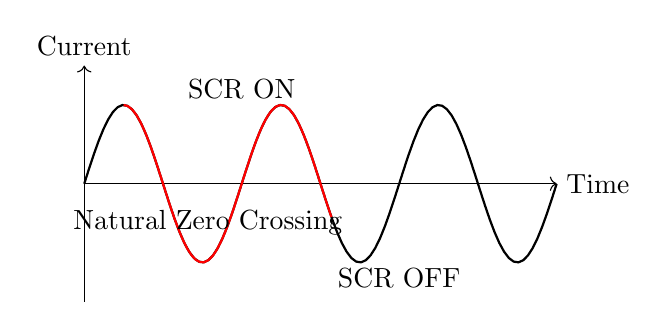
\begin{tikzpicture}
    \draw[->] (0,0) -- (6,0) node[right] {Time};
    \draw[->] (0,-1.5) -- (0,1.5) node[above] {Current};
    \draw[thick] plot[domain=0:6, samples=100] (\x, {sin(\x*180)});
    % Highlight conduction
    \draw[thick, red] plot[domain=0.5:3.14, samples=50] (\x, {sin(\x*180)});
    \node at (2,1.2) {SCR ON};
    \node at (4,-1.2) {SCR OFF};
    \node at (1.57, -0.5) {Natural Zero Crossing};
\end{tikzpicture}
\end{center}

\begin{itemize}
    \item \textbf{Definition}: SCR turns off automatically when current falls below holding current
    \item \textbf{AC circuit}: Occurs naturally at end of each positive half-cycle
    \item \textbf{Zero crossing}: SCR turns off when AC voltage crosses zero
    \item \textbf{No external circuit}: No additional components needed for turn-off
\end{itemize}

\begin{mnemonicbox}
"NAZC" (Natural At Zero Crossing)
\end{mnemonicbox}
\end{solutionbox}

\questionmarks{3(c)}{7}{Explain how TRIAC can be used as fan regulator and on-off control for ac power.}

\begin{solutionbox}
TRIAC is a bidirectional device ideal for AC power control applications.

\textbf{TRIAC Fan Regulator Circuit:}
\begin{center}
\begin{circuitikz}[american]
    \draw (0,0) to[sV, l=AC Source] (0,3) -- (2,3) to[L, l=Fan Motor] (4,3);
    \draw (4,3) to[triac, n=T, mirror] (4,0) -- (0,0);
    
    % Triggering
    \draw (2,3) -- (2,1.5) to[vR, l=$R$] (2,0.5) to[C, l=$C$] (4,0.5) -- (4,0);
    \draw (2,0.5) to[generic, l=DIAC] (T.G); % Use generic for diac to be safe
\end{circuitikz}
\end{center}

\textbf{TRIAC On-Off Control:}
\begin{center}
\begin{circuitikz}[american]
    \draw (0,0) to[sV, l=AC] (0,3) -- (2,3) to[R, l=Load] (4,3);
    \draw (4,3) to[triac, n=T, mirror] (4,0) -- (0,0);
    \draw (2,3) -- (2,1.5) to[R] (2,1) to[switch, l=Select] (T.G);
\end{circuitikz}
\end{center}

\begin{itemize}
    \item \textbf{Fan Regulation}: Phase control technique varies power to fan
    \item \textbf{Potentiometer}: Adjusts firing angle of TRIAC
    \item \textbf{On-Off Control}: Simple switch triggers TRIAC gate
    \item \textbf{Bidirectional}: Controls current in both half-cycles
\end{itemize}

\begin{mnemonicbox}
"FPOB" (Fan Power is controlled by Phase angle in both directions)
\end{mnemonicbox}
\end{solutionbox}

\vspace{0.5em}\centerline{\textbf{OR}}\questionmarks{3(a)}{3}{Draw symbol of SCR, DIAC and TRIAC.}

\begin{solutionbox}
\begin{center}
\begin{circuitikz}[american, scale=1.2, transform shape]
    % SCR
    \draw (0,2) to[thyristor, n=scr] (0,0);
    \node at (0, 2.5) {\textbf{SCR}};
    \node at (0, 2) [left] {A};
    \node at (0, 0) [left] {K};
    \node at (scr.gate) [right] {G};

    % DIAC (Manual drawing as fallback)
    \node at (4, 2.5) {\textbf{DIAC}};
    \draw (4, 2) -- (4, 1.6);
    \draw (4, 0.4) -- (4, 0);
    \draw (3.6, 1.6) -- (4.4, 1.6) -- (4, 0.8) -- (3.6, 1.6); % Down
    \draw (3.6, 0.8) -- (4.4, 0.8) -- (4, 1.6) -- (3.6, 0.8); % Up
    \draw (3.6, 0.8) -- (4.4, 0.8); % Bottom line of Up triangle
    \node at (4, 2) [left] {A1};
    \node at (4, 0) [left] {A2};

    % TRIAC
    \draw (8,2) to[triac, n=triac] (8,0);
    \node at (8, 2.5) {\textbf{TRIAC}};
    \node at (8, 2) [left] {MT2};
    \node at (8, 0) [left] {MT1};
    \node at (triac.gate) [right] {G};
\end{circuitikz}
\end{center}

\begin{mnemonicbox}
"SDT" (SCR has gate on one side, DIAC has none, TRIAC has gate in middle)
\end{mnemonicbox}
\end{solutionbox}

\questionmarks{3(b)}{4}{Draw and explain Gate triggering of SCR.}

\begin{solutionbox}
Gate triggering is the most common method to turn on an SCR.

\begin{center}
\begin{circuitikz}[american]
    \draw (0,0) to[sV, l=AC] (0,3) -- (2,3) to[thyristor, l=SCR, n=scr] (4,3) -- (4,0) to[R, l=Load] (2,0) -- (0,0);
    
    % Gate trigger circuit
    \draw (scr.gate) -- (2.5, 2.25) to[switch, l=SW] (2.5, 1.5) to[battery1, l=Example DC] (2.5, 0.5) -- (2.5, 0) node[ground]{}; % Simplified conceptual diagram
    % Connecting ground to cathode implicitly via load loop bottom?
    % Let's make it clearer.
\end{circuitikz}
\end{center}

\begin{itemize}
    \item \textbf{Principle}: Applying positive voltage between gate and cathode
    \item \textbf{Current requirement}: Small gate current triggers much larger anode current
    \item \textbf{Latching}: Once triggered, SCR remains ON even if gate signal is removed
    \item \textbf{Turn-off}: Requires reducing anode current below holding current
\end{itemize}

\begin{mnemonicbox}
"GPLT" (Gate Pulse Latches Thyristor)
\end{mnemonicbox}
\end{solutionbox}

\questionmarks{3(c)}{7}{Draw Construction and Voltage Vs Current characteristic of SCR and explain V-I characteristic.}

\begin{solutionbox}
SCR (Silicon Controlled Rectifier) is a four-layer PNPN semiconductor device.

\textbf{SCR Construction:}
\begin{center}
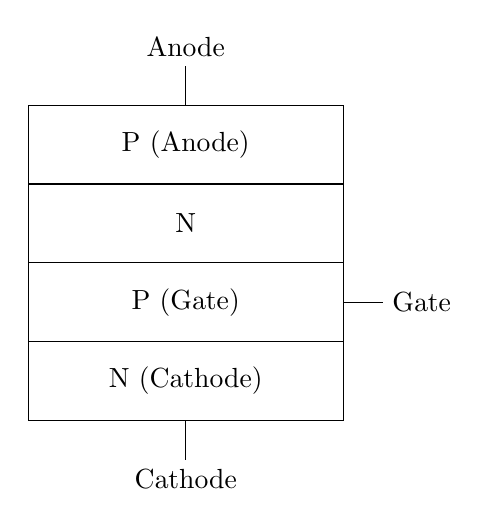
\begin{tikzpicture}
    % Layers
    \draw (0,0) rectangle (4,1) node[midway] {N (Cathode)};
    \draw (0,1) rectangle (4,2) node[midway] {P (Gate)};
    \draw (0,2) rectangle (4,3) node[midway] {N};
    \draw (0,3) rectangle (4,4) node[midway] {P (Anode)};
    
    % Terminals
    \draw (2,4) -- (2,4.5) node[above] {Anode};
    \draw (2,0) -- (2,-0.5) node[below] {Cathode};
    \draw (4,1.5) -- (4.5,1.5) node[right] {Gate};
\end{tikzpicture}
\end{center}

\textbf{V-I Characteristic:}
\begin{center}
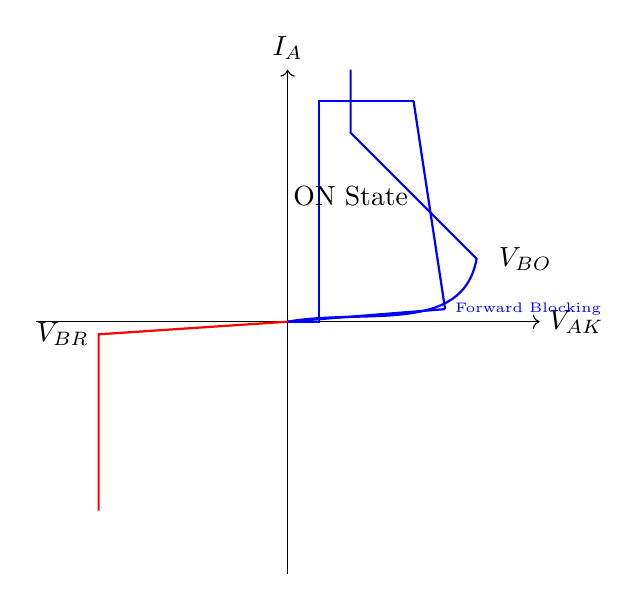
\begin{tikzpicture}[scale=0.8]
    \draw[->] (-4,0) -- (4,0) node[right] {$V_{AK}$};
    \draw[->] (0,-4) -- (0,4) node[above] {$I_A$};
    
    % Forward Blocking
    \draw[thick, blue] (0,0) -- (2.5,0.2) node[right, font=\tiny] {Forward Blocking};
    % Breakover
    \draw[thick, blue] (2.5,0.2) -- (2,3.5);
    % Conduction
    \draw[thick, blue] (2,3.5) -- (0.5,3.5) -- (0.5,0) -- (0,0); % Idealish latching
    % Let's draw standard curve
    \draw [blue, thick] (0,0) to[out=10, in=260] (3,1) -- (1,3) -- (1,4); 
    \node at (3.2, 1) [right] {$V_{BO}$};
    
    % Reverse
    \draw [red, thick] (0,0) -- (-3, -0.2) -- (-3, -3);
    \node at (-3, -0.2) [left] {$V_{BR}$};
    
    \node at (1, 2) {ON State};
\end{tikzpicture}
\end{center}

\begin{itemize}
    \item \textbf{Forward blocking region}: SCR conducts minimal current until breakover voltage
    \item \textbf{Forward conduction region}: Low resistance state after triggering
    \item \textbf{Reverse blocking region}: Blocks current in reverse direction
    \item \textbf{Gate triggering}: Reduces breakover voltage, facilitating turn-on
\end{itemize}

\begin{mnemonicbox}
"FBRH" (Forward Blocking, Reverse blocking, Holding current)
\end{mnemonicbox}
\end{solutionbox}
\questionmarks{4(a)}{3}{Explain OP-AMP as a summing amplifier.}

\begin{solutionbox}
Summing amplifier adds multiple input signals with weighted gains.

\begin{center}
\begin{circuitikz}[american, scale=1.0, transform shape]
    \node [op amp] (A) at (2,0) {};
    \draw (A.-) -- (0.5, 0.5) -- (0.5, 2);
    
    % Inputs
    \draw (0.5, 2) to[R, l=$R_1$] (-2, 2) node[left] {$V_1$};
    \draw (0.5, 1) to[R, l=$R_2$, *-] (-2, 1) node[left] {$V_2$};
    \draw (0.5, 0.5) to[short, *-] (0.5, 1);
    \draw (0.5, 0.5) -- (0.5, 0) to[R, l=$R_3$] (-2, 0) node[left] {$V_3$};
    
    \draw (A.+) -- (0.5, -0.5) to[short] (0.5,-1) node[ground] {};
    
    % Feedback
    \draw (A.-) -- (0.5, 0.5) -- (0.5, 3) to[R, l=$R_f$] (3.5, 3) -- (3.5, 0) -- (A.out);
    \draw (A.out) to[short, -o] (4,0) node[right] {$V_{out}$};
\end{circuitikz}
\end{center}

\begin{itemize}
    \item \textbf{Function}: Outputs weighted sum of input voltages
    \item \textbf{Output equation}: $V_{out} = -(V_1 \cdot \frac{R_f}{R_1} + V_2 \cdot \frac{R_f}{R_2} + V_3 \cdot \frac{R_f}{R_3})$
    \item \textbf{Equal weights}: When $R_1 = R_2 = R_3$, output is simple sum multiplied by $-R_f/R$
    \item \textbf{Virtual ground}: Inverting input maintains 0V potential
\end{itemize}

\begin{mnemonicbox}
"SWAP" (Sum Weighted And Proportional)
\end{mnemonicbox}
\end{solutionbox}

\questionmarks{4(b)}{4}{Define the following OP-AMP parameters: 1. input bias current 2. CMRR}

\begin{solutionbox}
\textbf{Input Bias Current}:
The average of the currents flowing into the two input terminals of an op-amp when the output is at zero.

\textbf{CMRR (Common Mode Rejection Ratio)}:
The ratio of differential gain to common-mode gain, indicating how well an op-amp rejects signals common to both inputs.

\begin{center}
\captionof{table}{Op-Amp Parameters}
\begin{tabulary}{\linewidth}{|L|L|L|}
\hline
\textbf{Parameter} & \textbf{Typical Value} & \textbf{Importance} \\
\hline
\textbf{Input Bias Current} & 20-200 nA & Lower is better for high impedance circuits \\
\hline
\textbf{CMRR} & 80-120 dB & Higher is better for noise rejection \\
\hline
\end{tabulary}
\end{center}

\begin{mnemonicbox}
"BIC-CMR" (Bias Is Current, Common Mode Rejection)
\end{mnemonicbox}
\end{solutionbox}

\questionmarks{4(c)}{7}{Draw and explain monostable multivibrator using 555 Timer.}

\begin{solutionbox}
Monostable multivibrator generates a single pulse of predetermined duration when triggered.

\begin{center}
\begin{circuitikz}[american, scale=0.9, transform shape]
    % 555 Timer Block
    \draw (0,0) rectangle (4,4);
    \node at (2,2) {555 Timer};
    
    % Pins
    \node at (0,3.5) [right] {8 (VCC)}; \draw (0,3.5) -- (-1,3.5) node[vcc] {$V_{CC}$};
    \node at (0,0.5) [right] {1 (GND)}; \draw (0,0.5) -- (-1,0.5) node[ground] {};
    
    \node at (4,2.5) [left] {3 (OUT)}; \draw (4,2.5) -- (5,2.5) node[right] {$V_{out}$};
    
    \node at (0,2.5) [right] {2 (TRIG)}; \draw (0,2.5) -- (-1,2.5) node[left] {Trigger};
    \node at (0,1.5) [right] {4 (RST)}; \draw (0,1.5) -- (-1,1.5) node[heading] {to VCC};
    
    % External components
    \node at (4,3.5) [left] {7 (DIS)}; \draw (4,3.5) -- (5,3.5) -- (5,4.5) to[R, l=$R$] (5,6) node[vcc] {$V_{CC}$};
    \node at (4,0.5) [left] {6 (THR)}; \draw (4,0.5) -- (5,0.5) -- (5,3.5); % Connect THR to DIS? No, connected to C usually.
    % Monostable: R connects VCC to DIS and THR. C connects THR/DIS to GND.
    % Correct:
    % Pin 7 (DIS) connected to junction of R and C?
    % Monostable: R from VCC to Pin 7 & 6. C from Pin 7 & 6 to GND.
    % Wait, standard is: VCC -> R -> Pin 7 and 6 -> C -> GND.
    
    % Let's correct standard Monostable 555
    \draw (4,3.5) -- (5,3.5); % Pin 7
    \draw (4,1.5) [left] node {6 (THR)}; \draw (4,1.5) -- (5,1.5) -- (5,3.5); % Pin 6 connected to 7
    \draw (5,3.5) to[R, l=$R$] (5,5.5) node[vcc] {$V_{CC}$};
    \draw (5,1.5) to[C, l=$C$] (5,-1) node[ground] {};
    
    % Pin 5 (CV) usually open or cap to ground
    % Pin 2 Trigger
\end{circuitikz}
\end{center}

\textbf{Output Waveform:}
\begin{center}
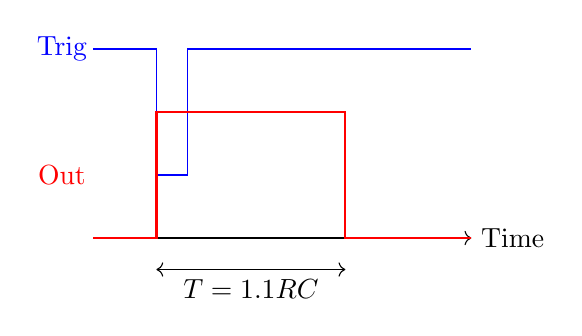
\begin{tikzpicture}[scale=0.8]
    \draw[->] (0,0) -- (6,0) node[right] {Time};
    
    % Trigger
    \draw[blue] (0,3) -- (1,3) -- (1,1) -- (1.5,1) -- (1.5,3) -- (6,3); 
    \node[blue] at (-0.5, 3) {Trig};
    
    % Output
    \draw[red, thick] (0,0) -- (1,0) -- (1,2) -- (4,2) -- (4,0) -- (6,0);
    \node[red] at (-0.5, 1) {Out};
    
    % Dimension
    \draw[<->] (1, -0.5) -- (4, -0.5) node[midway, below] {$T = 1.1 RC$};
\end{tikzpicture}
\end{center}

\begin{itemize}
    \item \textbf{Operation}: Single stable state (output LOW), temporarily HIGH when triggered
    \item \textbf{Pulse width}: $T = 1.1 \times R \times C$ (seconds)
    \item \textbf{Triggering}: Falling edge on TRIG pin (pin 2)
    \item \textbf{Timing components}: $R$ and $C$ determine pulse duration
\end{itemize}

\begin{mnemonicbox}
"POST" (Pulse Output, Single Trigger)
\end{mnemonicbox}
\end{solutionbox}

\vspace{0.5em}\centerline{\textbf{OR}}\questionmarks{4(a)}{3}{Draw the circuit diagram of OP-AMP as a inverting amplifier.}

\begin{solutionbox}
\begin{center}
\begin{circuitikz}[american, scale=1.0, transform shape]
    \node [op amp] (A) at (0,0) {};
    \draw (A.+) -- (-1, -0.5) node[ground] {};
    \draw (A.-) -- (-1, 0.5) to[R, l=$R_1$] (-3, 0.5) node[left] {$V_{in}$};
    \draw (A.-) -- (-1, 0.5) -- (-1, 1.5) to[R, l=$R_f$] (1, 1.5) -- (1, 0) -- (A.out);
    \draw (A.out) to[short, -o] (2,0) node[right] {$V_{out}$};
\end{circuitikz}
\end{center}

\begin{mnemonicbox}
"IRON" (Inverting Requires One Negative input)
\end{mnemonicbox}
\end{solutionbox}

\questionmarks{4(b)}{4}{Define the following OP-AMP parameters: 1. input offset current 2. slew rate}

\begin{solutionbox}
\textbf{Input Offset Current}:
The difference between the currents flowing into the two input terminals of an op-amp.

\textbf{Slew Rate}:
The maximum rate of change of output voltage per unit of time, typically measured in $V/\mu s$.

\begin{center}
\captionof{table}{Op-Amp Parameters}
\begin{tabulary}{\linewidth}{|L|L|L|}
\hline
\textbf{Parameter} & \textbf{Typical Value} & \textbf{Importance} \\
\hline
\textbf{Input Offset Current} & 2-50 nA & Lower is better for precision applications \\
\hline
\textbf{Slew Rate} & 0.5-20 V/$\mu$s & Higher is better for high-frequency operation \\
\hline
\end{tabulary}
\end{center}

\begin{mnemonicbox}
"IOSR" (Input Offset and Slew Rate)
\end{mnemonicbox}
\end{solutionbox}

\questionmarks{4(c)}{7}{Explain op-amp as Inverting amplifier and obtain equation of its Voltage gain.}

\begin{solutionbox}
Inverting amplifier produces an output signal that is inverted and amplified.

\begin{center}
\begin{circuitikz}[american, scale=1.0, transform shape]
    \node [op amp] (A) at (0,0) {};
    \draw (A.+) -- (-1, -0.5) node[ground] {};
    \draw (A.-) -- (-1, 0.5) to[R, l=$R_1$] (-3, 0.5) node[left] {$V_{in}$};
    \draw (A.-) -- (-1, 0.5) -- (-1, 1.5) to[R, l=$R_f$] (1, 1.5) -- (1, 0) -- (A.out);
    \draw (A.out) to[short, -o] (2,0) node[right] {$V_{out}$};
\end{circuitikz}
\end{center}

\textbf{Voltage Gain Derivation:}

At node N (inverting input):
$$ I_1 + I_f = 0 \quad (\text{By Kirchhoff's Current Law}) $$
$$ \frac{V_{in} - V_N}{R_1} + \frac{V_{out} - V_N}{R_f} = 0 $$

Since $V_N \approx 0$ (virtual ground):
$$ \frac{V_{in}}{R_1} + \frac{V_{out}}{R_f} = 0 $$
$$ \frac{V_{out}}{V_{in}} = -\frac{R_f}{R_1} $$

\begin{itemize}
    \item \textbf{Gain equation}: $V_{out}/V_{in} = -R_f/R_1$
    \item \textbf{Virtual ground}: Inverting terminal maintained at 0V
    \item \textbf{Input impedance}: Equal to $R_1$
    \item \textbf{Negative feedback}: Provides stability and linearity
\end{itemize}

\begin{mnemonicbox}
"GIVN" (Gain Is Negative, Virtual ground)
\end{mnemonicbox}
\end{solutionbox}
\questionmarks{5(a)}{3}{Draw the block diagram of IC 555.}

\begin{solutionbox}
\textbf{Block Diagram of IC 555:}

\begin{center}
\begin{tikzpicture}[gtu block]
    % Components:
    % Voltage Divider R-R-R
    \node (vcc) at (0,6) {$V_{CC} (8)$};
    \node [draw, rectangle] (r1) at (0,4.5) {5k$\Omega$};
    \node [draw, rectangle] (r2) at (0,3) {5k$\Omega$};
    \node [draw, rectangle] (r3) at (0,1.5) {5k$\Omega$};
    \node (gnd) at (0,0) {GND (1)};
    
    \draw (vcc) -- (r1) -- (r2) -- (r3) -- (gnd);
    
    % Comparators
    \node [draw, regular polygon, regular polygon sides=3, rotate=-90, inner sep=1pt] (comp1) at (3,4) {UC}; % Upper Comparator
    \node [draw, regular polygon, regular polygon sides=3, rotate=-90, inner sep=1pt] (comp2) at (3,2) {LC}; % Lower Comparator
    
    % Connections to Comparators
    \draw (0,4) -- (comp1.south) node[above left] {-}; % 2/3 VCC to Inverting of UC
    \draw (0,2) -- (comp2.north) node[below left] {+}; % 1/3 VCC to Non-Inverting of LC
    
    % Pins
    \node (thr) at (-2, 4) {Threshold (6)};
    \draw (thr) -- (comp1.north) node[above left] {+};
    
    \node (trig) at (-2, 2) {Trigger (2)};
    \draw (trig) -- (comp2.south) node[below left] {-};
    
    \node (ctrl) at (2, 5) {Control (5)};
    \draw (ctrl) |- (0, 4);
    
    % Flip Flop
    \node [draw, rectangle, minimum width=2cm, minimum height=1.5cm] (ff) at (6,3) {SR Flip-Flop};
    \draw (comp1.west) -- (ff.north west) node[below right] {R}; % Tip is West due to rotation? Wait. Rotate -90 points tip down?
    % Let's re-verify Triangle orientation.
    % Standard op-amp: tip is output.
    % If rotate -90, tip is RIGHT.
    % comp1.east is output.
    \draw (comp1.east) -- (ff.140); % Upper input (R)
    \draw (comp2.east) -- (ff.220); % Lower input (S)
    
    % Output Stage
    \node [draw, triangular amplifier] (inv) at (9,3) {Buffer};
    \draw (ff.east) -- (inv.west);
    \draw (inv.east) -- (11,3) node[right] {Output (3)};
    
    % Discharge Transistor
    \node [npn, rotate=0] (Q1) at (6, 0.5) {};
    \draw (Q1.E) -- (6,0) node[ground] {};
    \draw (Q1.C) -- (8,0.5) node[right] {Discharge (7)};
    \draw (Q1.B) -| (ff.300); % Qbar output likely drives discharge
    
    % Reset
    \node (rst) at (6, 5) {Reset (4)};
    \draw (rst) -- (ff.north);
\end{tikzpicture}
\end{center}

\begin{mnemonicbox}
"CVOT" (Comparators, Voltage divider, Output stage, Timer)
\end{mnemonicbox}
\end{solutionbox}

\questionmarks{5(b)}{4}{Draw the circuit diagram of OP-AMP as a wein bridge oscillator.}

\begin{solutionbox}
\textbf{Wein Bridge Oscillator Circuit:}

\begin{center}
\begin{circuitikz}[american, scale=1.0, transform shape]
    \node [op amp] (A) at (0,0) {};
    
    % Feedback Network (Wein Bridge)
    % Series RC
    \draw (A.+) -- (-1, -0.5) -- (-1, -1.5);
    \draw (-1, -1.5) to[R, l=$R_1$] (-1, -3) to[C, l=$C_1$] (-1, -4.5) node[ground] {}; % Wait, Series RC is usually top arm?
    % Standard Wein Bridge:
    % Series RC from Vout to Non-Inverting input.
    % Parallel RC from Non-Inverting input to Ground.
    
    % Let's fix.
    \draw (A.out) -- (1,0) -- (1, -4) -- (-3, -4) -- (-3, -1) to[R, l=$R$] (-3, 0.5) to[C, l=$C$] (-1, 0.5) -- (A.+); % Feedback path
    % No, that's messy.
    
    % Better layout:
    % Op Amp
    \draw (A.out) to[short, -o] (2,0) node[right] {$V_{out}$};
    
    % Positive Feedback (Lead-Lag)
    \draw (2,0) -- (2, 2) -- (-2, 2) to[C, l=$C$] (-4, 2) to[R, l=$R$] (-4, 0) -- (A.+); % Series arm
    \draw (-4, 0) to[R, l=$R$] (-4, -2) node[ground] {}; % Parallel R
    \draw (-2.5, 0) to[C, l=$C$] (-2.5, -2) node[ground] {}; % Parallel C (connected in parallel to R at node)
    \draw (-4,0) -- (-2.5,0); % Connect parallel components
    
    % Negative Feedback (Gain setting)
    \draw (A.-) -- (-1, 0.5) to[R, l=$R_3$] (-1, 2.5) -- (1, 2.5) -- (1,0); % Rf usually
    \draw (A.-) -- (-1, 0.5) to[R, l=$R_4$] (-1, -1.5) node[ground] {};
    
\end{circuitikz}
\end{center}

\begin{mnemonicbox}
"WPRC" (Wein Produces Resonant Circuit)
\end{mnemonicbox}
\end{solutionbox}

\questionmarks{5(c)}{7}{Explain working of different types of Fixed and variable voltage regulator IC.}

\begin{solutionbox}
Voltage regulator ICs maintain stable output voltage despite input or load variations.

\textbf{Fixed Voltage Regulators:}
\begin{center}
\begin{circuitikz}[american, scale=0.9, transform shape]
    \draw (0,0) rectangle (3,2);
    \node at (1.5,1) {78XX};
    \draw (-1,1.5) to[short, o-] (0,1.5) node[above left] {IN};
    \draw (3,1.5) to[short, -o] (4,1.5) node[above right] {OUT};
    \draw (1.5,0) -- (1.5,-1) node[ground] {} node[right] {GND};
    
    \draw (-1,1.5) to[C, l=$C_{in}$] (-1,0) node[ground] {};
    \draw (4,1.5) to[C, l=$C_{out}$] (4,0) node[ground] {};
\end{circuitikz}
\end{center}

\textbf{Variable Voltage Regulator:}
\begin{center}
\begin{circuitikz}[american, scale=0.9, transform shape]
    \draw (0,0) rectangle (3,2);
    \node at (1.5,1) {LM317};
    \draw (-1,1.5) to[short, o-] (0,1.5) node[above left] {IN};
    \draw (3,1.5) to[short, -o] (4,1.5) node[above right] {OUT};
    \draw (1.5,0) -- (1.5,-0.5) node[right] {ADJ};
    
    \draw (-1,1.5) to[C, l=$C_{in}$] (-1,0) node[ground] {};
    
    % Adj resistors
    \draw (1.5,-0.5) to[R, l=$R_2$] (1.5,-2.5) node[ground] {};
    \draw (1.5,-0.5) -- (4, -0.5) -- (4, 1.5);
    \draw (4, 0.5) to[R, l=$R_1$] (1.5, 0.5); % Resistor between OUT and ADJ? 
    % LM317: R1 between OUT and ADJ. R2 between ADJ and GND.
    % Fix:
    \draw (3,1.5) -- (3.5,1.5) to[R, l=$R_1$] (3.5,-0.5) -- (1.5,-0.5);
    \draw (4,1.5) to[C, l=$C_{out}$] (4,0) node[ground] {};
\end{circuitikz}
\end{center}

\begin{itemize}
    \item \textbf{Fixed regulators}: 78XX (positive) and 79XX (negative) series provide specific voltages
    \item \textbf{Variable regulators}: LM317 (positive) and LM337 (negative) allow adjustable output
    \item \textbf{Three-terminal design}: Input, output, and ground/adjust terminals
    \item \textbf{Output equation for LM317}: $V_{out} = 1.25V \times (1 + R_2/R_1)$
    \item \textbf{Protection features}: Short circuit, thermal overload, and safe area protection
\end{itemize}

\begin{mnemonicbox}
"FAVOR" (Fixed And Variable Output Regulators)
\end{mnemonicbox}
\end{solutionbox}

\vspace{0.5em}\centerline{\textbf{OR}}\questionmarks{5(a)}{3}{Draw the block diagram of astable multivibrator using 555 timer.}

\begin{solutionbox}
\textbf{Astable Multivibrator Block Diagram:}

\begin{center}
\begin{tikzpicture}[gtu block]
    % 555 Box
    \draw [dashed] (-1,-1) rectangle (5,5);
    \node at (4.5,4.5) {555};
    
    % Components within 555 connected externally for astable
    % Actually Question asks for BLOCK DIAGRAM of Astable using 555
    % Usually means showing 555 block + external R1, R2, C
    
    \node [draw, rectangle, minimum width=2cm, minimum height=3cm] (ic) at (2,2) {555 Timer};
    
    % Pins
    \node (vcc) at (2,4.5) {8 (VCC)};
    \draw (ic.north) -- (vcc);
    
    \node (gnd) at (2,-0.5) {1 (GND)};
    \draw (ic.south) -- (gnd);
    
    \draw (ic.west) ++(0, 1) -- ++(-1,0) node[left] {7 (DIS)};
    \draw (ic.west) ++(0, 0) -- ++(-1,0) node[left] {6 (THR)};
    \draw (ic.west) ++(0, -1) -- ++(-1,0) node[left] {2 (TRIG)};
    
    \draw (ic.east) -- ++(1,0) node[right] {3 (OUT)};
    
    % External Circuit
    \draw (-3, 5) node[vcc] {$V_{CC}$} to[R, l=$R_1$] (-3, 3) -- (1, 3); % To DIS (7)
    \draw (-3, 3) to[R, l=$R_2$] (-3, 1) -- (1, 1); % To THR (6)
    \draw (-3, 1) -- (-3, 0) -- (1, 0); % To TRIG (2) shorted to 6
    \draw (-3, 0) to[C, l=$C$] (-3, -2) node[ground] {};
    
    \draw (1,3) -- (0.8,3); % Connect to wire
    \draw (1,1) -- (0.8,1);
    \draw (1,0) -- (0.8,0);
\end{tikzpicture}
\end{center}

\begin{mnemonicbox}
"FOFT" (Free-running Oscillator From Timer)
\end{mnemonicbox}
\end{solutionbox}

\questionmarks{5(b)}{4}{Draw and explain solar based battery charger circuits.}

\begin{solutionbox}
Solar battery charger converts solar energy to charge batteries.

\begin{center}
\begin{circuitikz}[american, scale=1.0, transform shape]
    \draw (0,0) to[pvsource, l=Solar Panel] (0,3);
    \draw (0,3) to[D, l=Blocking Diode] (3,3) to[generic, l=Regulator IC] (5,3);
    \draw (5,3) to[battery, l=Battery] (5,0) -- (0,0);
    
    % Charge Indicator LED
    \draw (4,3) to[led, l=LED] (4,0) node[ground] {}; % Simplified
\end{circuitikz}
\end{center}

\begin{itemize}
    \item \textbf{Solar panel}: Converts sunlight to DC electricity
    \item \textbf{Blocking diode}: Prevents battery discharge through panel at night
    \item \textbf{Regulator IC}: Controls charging voltage and current
    \item \textbf{Charge indicator}: Shows charging status
    \item \textbf{Protection}: Overcharge and reverse polarity protection
\end{itemize}

\begin{mnemonicbox}
"SBRCP" (Solar, Blocking diode, Regulator, Charging, Protection)
\end{mnemonicbox}
\end{solutionbox}

\questionmarks{5(c)}{7}{Draw and explain the block diagram of SMPS.}

\begin{solutionbox}
SMPS (Switch Mode Power Supply) converts electrical power efficiently using switching regulators.

\begin{center}
\begin{tikzpicture}[gtu block]
    \node (ac) [draw, rectangle] {AC Input};
    \node (rect1) [draw, rectangle, right=0.5cm of ac] {Input Rectifier \& Filter};
    \node (switch) [draw, rectangle, right=0.5cm of rect1] {High Freq Switch};
    \node (trans) [draw, rectangle, right=0.5cm of switch] {Power Transformer};
    \node (rect2) [draw, rectangle, below=1cm of trans] {Output Rectifier \& Filter};
    \node (load) [draw, rectangle, left=0.5cm of rect2] {Load};
    \node (ctrl) [draw, rectangle, left=0.5cm of load] {Control Circuit};
    
    \draw [gtu arrow] (ac) -- (rect1);
    \draw [gtu arrow] (rect1) -- (switch);
    \draw [gtu arrow] (switch) -- (trans);
    \draw [gtu arrow] (trans) -- (rect2);
    \draw [gtu arrow] (rect2) -- (load);
    \draw [gtu arrow] (load) -- (ctrl);
    \draw [gtu arrow] (ctrl) -| (switch);
\end{tikzpicture}
\end{center}

\begin{itemize}
    \item \textbf{Input Stage}: Rectifies and filters AC mains to high voltage DC
    \item \textbf{Switching}: Chops DC into high-frequency AC pulse train
    \item \textbf{Transformer}: Steps down/up voltage and provides isolation
    \item \textbf{Output Stage}: Rectifies and filters high-frequency AC to flat DC
    \item \textbf{Feedback}: Compares output to reference for PWM control
\end{itemize}

\begin{mnemonicbox}
"IRS-TOF" (Input, Rectifier, Switching, Transformer, Output, Feedback)
\end{mnemonicbox}
\end{solutionbox}

\end{document}
